\section{Example}
\label{subsec:example}
%Step-by-step example (intention is to move this to an appendix)
Here, a contrived Hamiltonian is used to show the step-by-step procedure of LOBE. The example Hamiltonian, with a bosonic occupancy cutoff $\Omega = 3$, that will be used is 

\begin{equation}
    H = b_0^\dagger d_0(a_0^\dagger)^2 + 2 d_0^\dagger a_0^\dagger a_0+3 b_0^\dagger d_0^\dagger d_0
\end{equation}

\textbf{Step 1: Rescale Hamiltonian from bosonic terms:}
Via equation \ref{bose coeff rescale}, $\frac{1}{(\Omega + 1)^{K/2}} = \frac{1}{4}$ because $K = 2$ (there are at most 2 bosonic creation/annihilation terms, which in this case come from the first term). Now the Hamiltonian becomes 
\begin{equation}
    H^* = \frac{1}{4}H
\end{equation}

\textbf{Step 2: Rescale coefficients of Hamiltonian (assuming USP):} In order to load the Hamiltonian coefficients into the circuit via the $R_y$ gates in the \textit{coefficient} oracle, we need to ensure the coefficients are $\leq 1$. This is done via equation \ref{usp scale}. 
In this case, $L = 3$ since there are three terms, and $\alpha^* = 3$, the largest term coefficient. Thus, $\lambda_{usp} = 12$. Now, via \ref{Hbar scale}, the fully rescaled Hamiltonian is:
\begin{equation}
    \bar{H} = \frac{1}{48}b_0^\dagger d_0(a_0^\dagger)^2 + \frac{1}{24} d_0^\dagger a_0^\dagger a_0+\frac{1}{16} b_0^\dagger d_0^\dagger d_0
\end{equation}

\textbf{Step 3: Obtain the corresponding LOBE circuit:} In the style of figure \ref{fig:select-normal-ordering}, for this particular Hamiltonian, the three \textit{select} oracle unitaries: $U_{T_0}, U_{T_1}, U_{T_2}$ appear as:
\begin{figure}[h]
    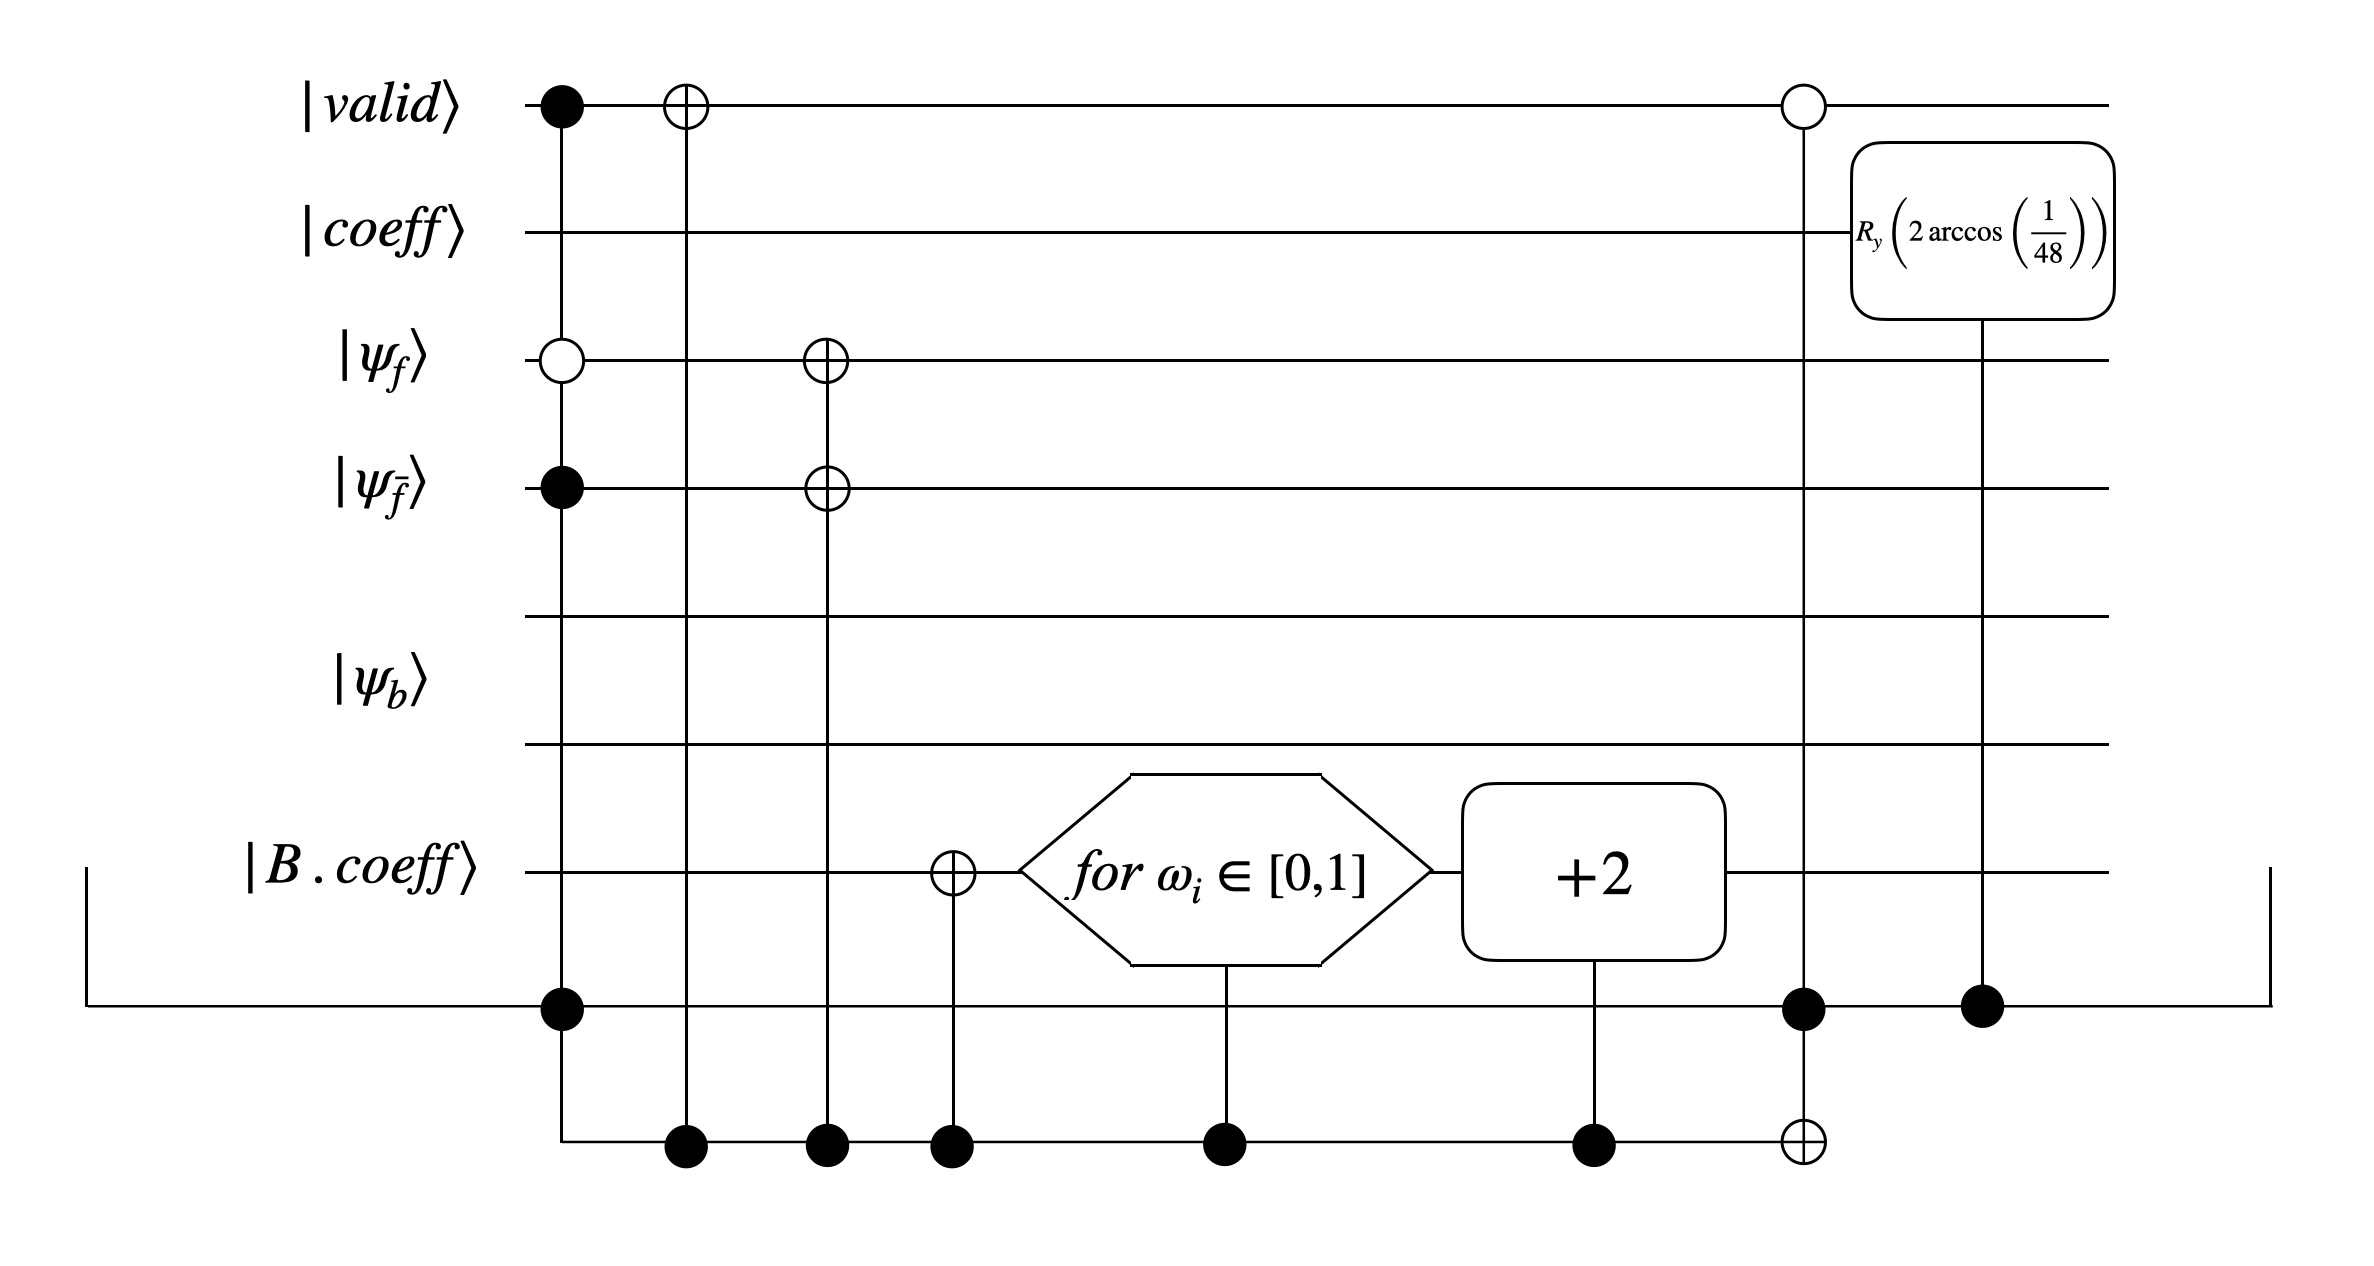
\includegraphics[width = 0.7\linewidth]{figures/T0.png}
    \caption{\textit{Select} unitary $U_{T_0}$ that block-encodes $T_0 = \frac{1}{48}b_0^\dagger d_0(a_0^\dagger)^2$}
\end{figure}
\begin{figure}[h]
    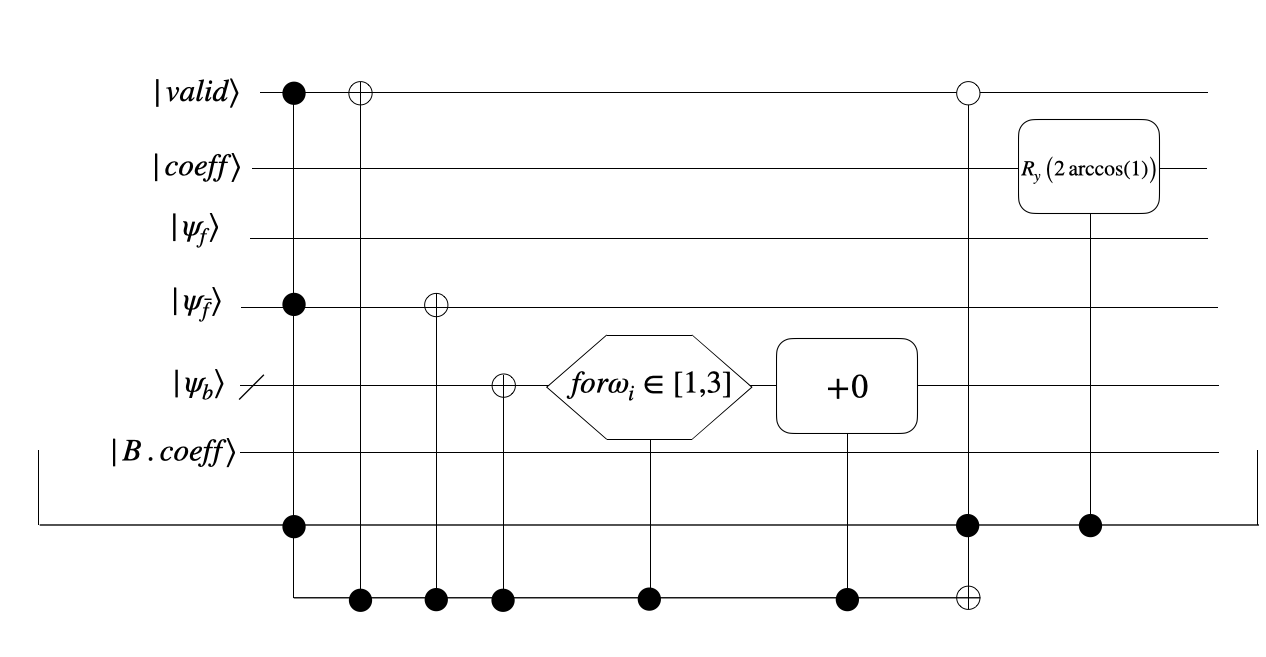
\includegraphics[width = 0.7\linewidth]{figures/T1.png}
    \caption{\textit{Select} unitary $U_{T_1}$ that block-encodes $T_1 = \frac{1}{24}a_0^\dagger a_0 d_0^\dagger$}
\end{figure}
\begin{figure}[h]
    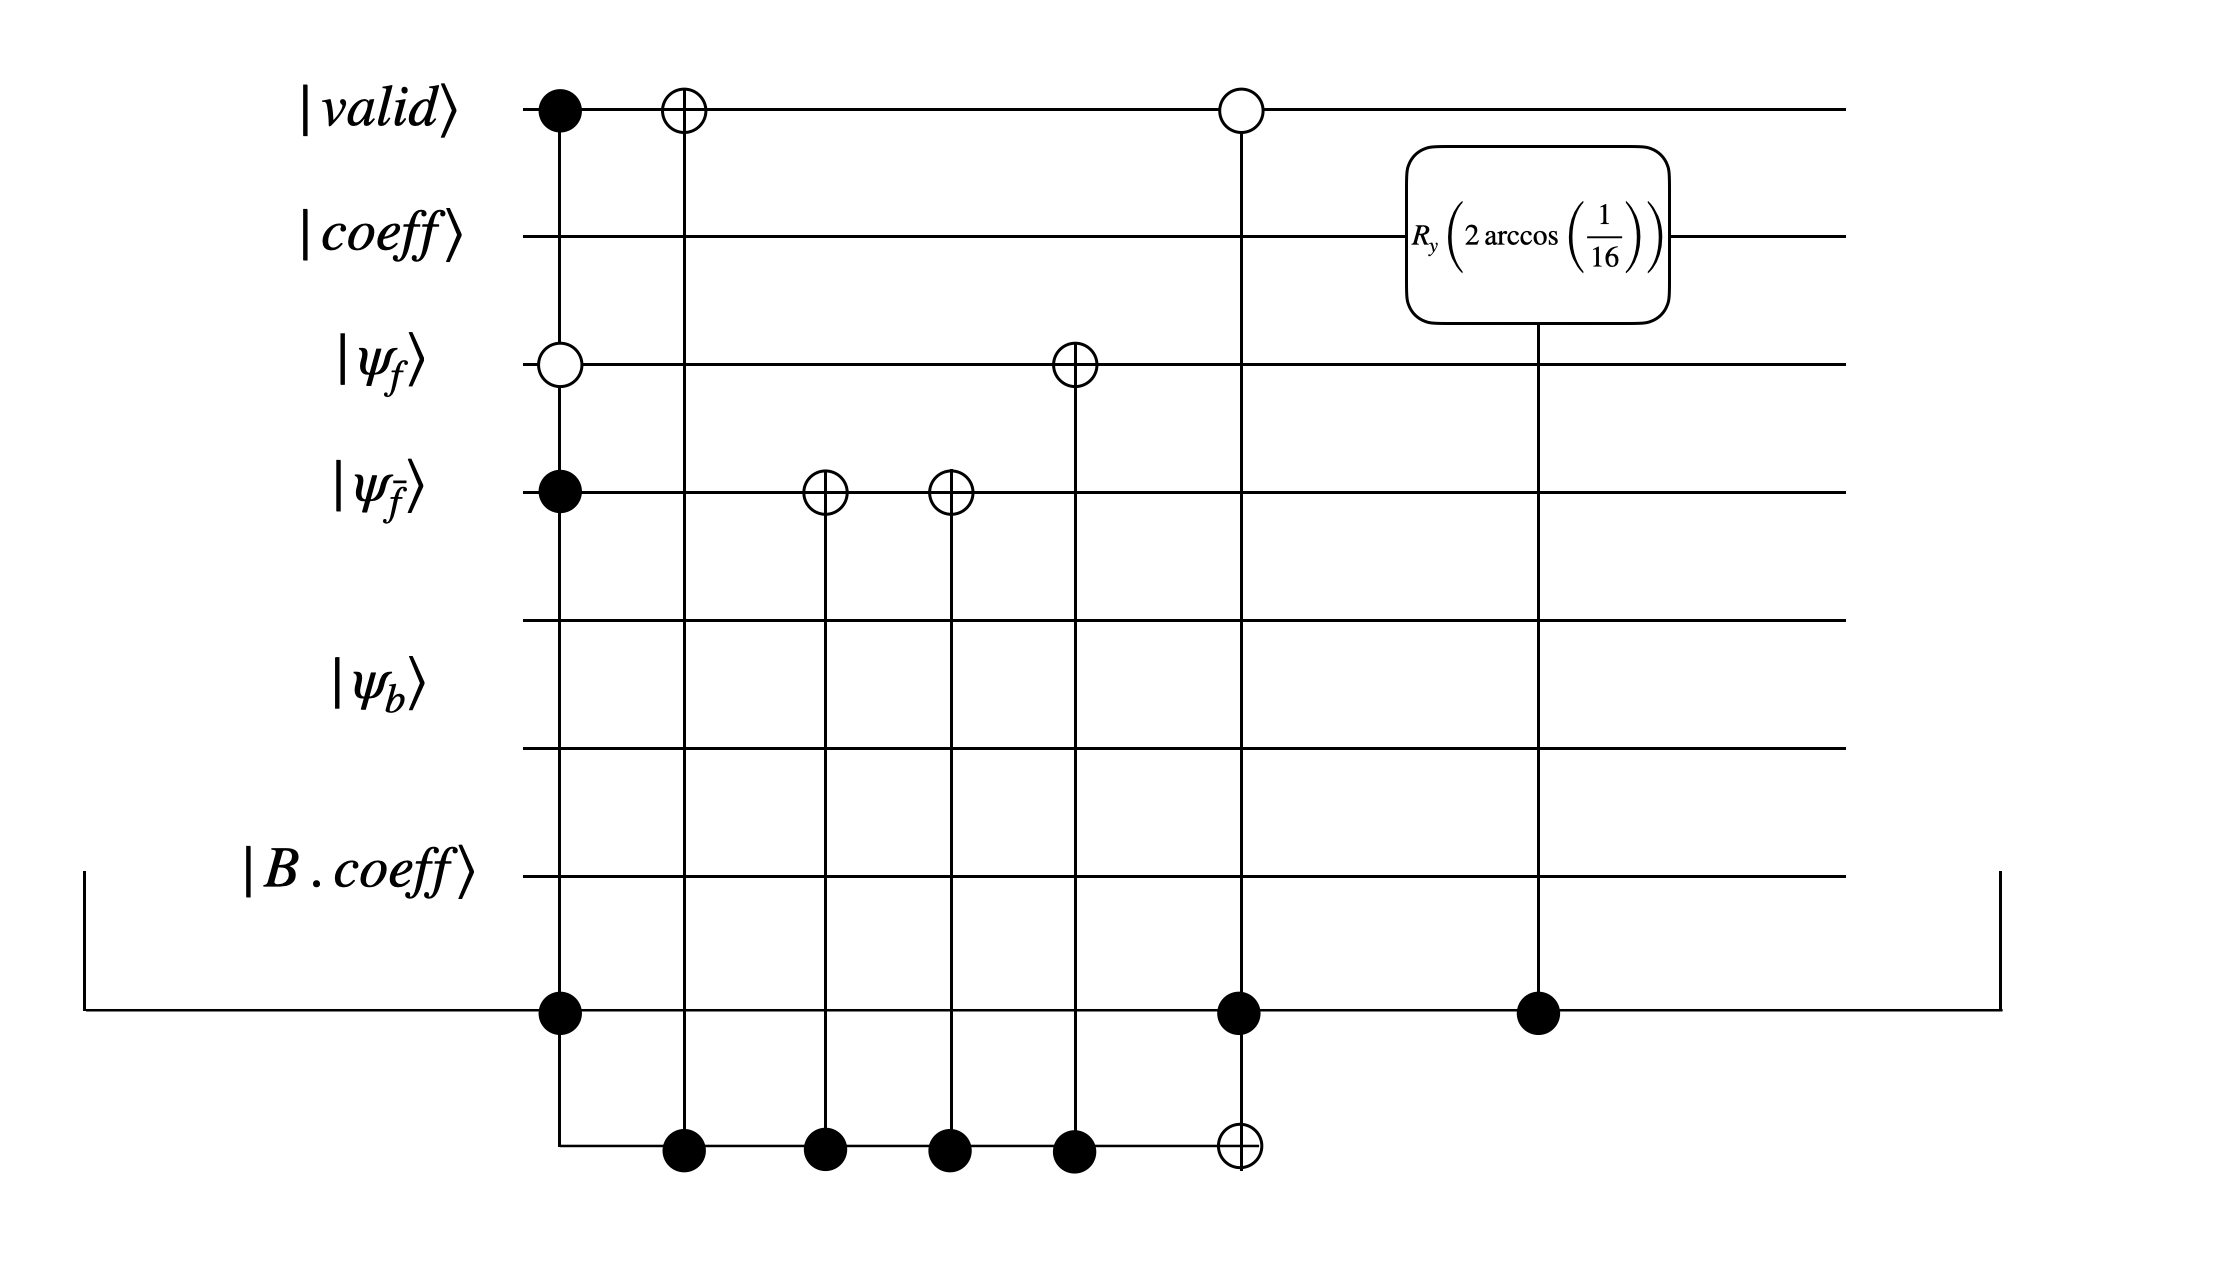
\includegraphics[width = 0.7\linewidth]{figures/T2.png}
    \caption{\textit{Select} unitary $U_{T_2}$ that block-encodes $T_2 = \frac{1}{16}b_0^\dagger d_0^\dagger d_0$}
\end{figure}

\textbf{Step 4: Count gates:} Using the notation in \ref{count gates not.}, the preceeding three unitaries have the following gate counts:

\begin{align}
    C_{U_{T_0}} &= (3, 1, 5, 5)\\
    C_{U_{T_1}} &= (4, 1, 5, 5)\\
    C_{U_{T_2}} &= (1, 1, 3, 3)
\end{align}
Thus, the total cost of the \textit{select} oracle is $C_{\textit{select}} = (8, 3, 13, 13)$. 

\textbf{Step 5: Post-process the eigenvalues:} After obtaining the full block-encoding of the Hamiltonian, the eigenvalues (which can be obtained via phase estimation) must be post-processed. This is because the eigenvalues of the block encoded Hamiltonian will correspond to $\bar{H}$, \textit{not} $H$ (the original problem Hamiltonian).
For this example, $\bar{H} = \frac{1}{48}H$, so if eigenvalues of the block Hamiltonian are obtained as $\bar{E}_i$, then $\bar{E_i} = \frac{1}{48}E_i$. Thus,
\begin{equation}
    E_i = 48\bar{E}_i
\end{equation}